This chapter shows the main results obtained. On section one we present the quantitative
performance and training results. Section 2 explains how the different visualizations
are generated, including examples for all the models.

\section{Quantitative results}

\subsection{Model performance}

Even though the objective of this research is to learn a ranking (or regression) to
quantify the urban perception, exact labels for this are not available, so we have to measure
model performance based on the Place Pulse votes, which as was mentioned on section
\ref{sec:problem_def}, has considerable issues. We use as performance measure the
equivalent to classification accuracy, considering which image won the vote as the target label.
In other words, we evaluate the percentage of restrictions (see \ref{eq:constraints})
that are satisfied by the model. We do this separately for each attribute in it's corresponding
validation set and the final accuracy value for each model is calculated as the mean accuracy through
all attributes.

Both ResNet based baseline models achieve an accuracy of \texttildelow 66\% and
as it was expected, replacing the more expressive CNN features for semantic segmentation,
caused a significant performance drop, falling to 60.62\% for SegRank and 61.44\%
for SelfSegRank. The performance is then mostly recovered when combining both approaches,
reaching 64.41\% on the AttentionSegRank arquitecture. See table \ref{tab:model_acc}, for the exact accuracy values.


\begin{table}[H]
	\caption[Model accuracy]{Accuracy values for each model on all attributes.}
	\begin{tabular}{|l|r|r|r|r|r|}
		\hline
		Attibute/Model & Resnet50 & ResnetAttn & SegRank & SelfSegRank  & AttnSegRank \\ \hline
		Wealthy        & 68.45\%   & 68.60\%    & 60.99\% & 61.89\%     & 66.27\%     \\
		Depressing     & 65.87\%   & 66.02\%    & 61.73\% & 62.30\%     & 64.33\%     \\
		Safety         & 65.41\%   & 65.46\%    & 59.08\% & 60.24\%     & 64.04\%     \\
		Lively         & 65.93\%   & 64.78\%    & 58.96\% & 60.29\%     & 63.35\%     \\
		Boring         & 62.28\%   & 62.20\%    & 58.01\% & 58.51\%     & 61.06\%     \\
		Beautiful      & 70.02\%   & 69.60\%    & 64.93\% & 65.43\%     & 67.99\%     \\ \hline
		Average        & \textbf{66.33\%}    & 66.11\%    & 60.62\% & 61.44\%     & 64.51\%     \\ \hline
	\end{tabular}
	\label{tab:model_acc}
\end{table}

\subsection{Training behavior}
\label{sec:training}

Models trained on the place pulse dataset are very prone to overfitting, we believe this is due to it
having a very large amount of votes in comparison to the amount of available images, and because the task
is very hard to generalize given the high amount of noise that the dataset has from how it was collected.
This can be seen clearly on figures \ref{fig:resnet_graph} and \ref{fig:resnet_attn_graph}. Both
baselines models present considerable overfitting, showing accuracy differences between seen and unseen data
of up to 25\%, and ceasing to improve on the validation set after one or two training epochs.

\begin{figure}[ht]
	\begin{center}
	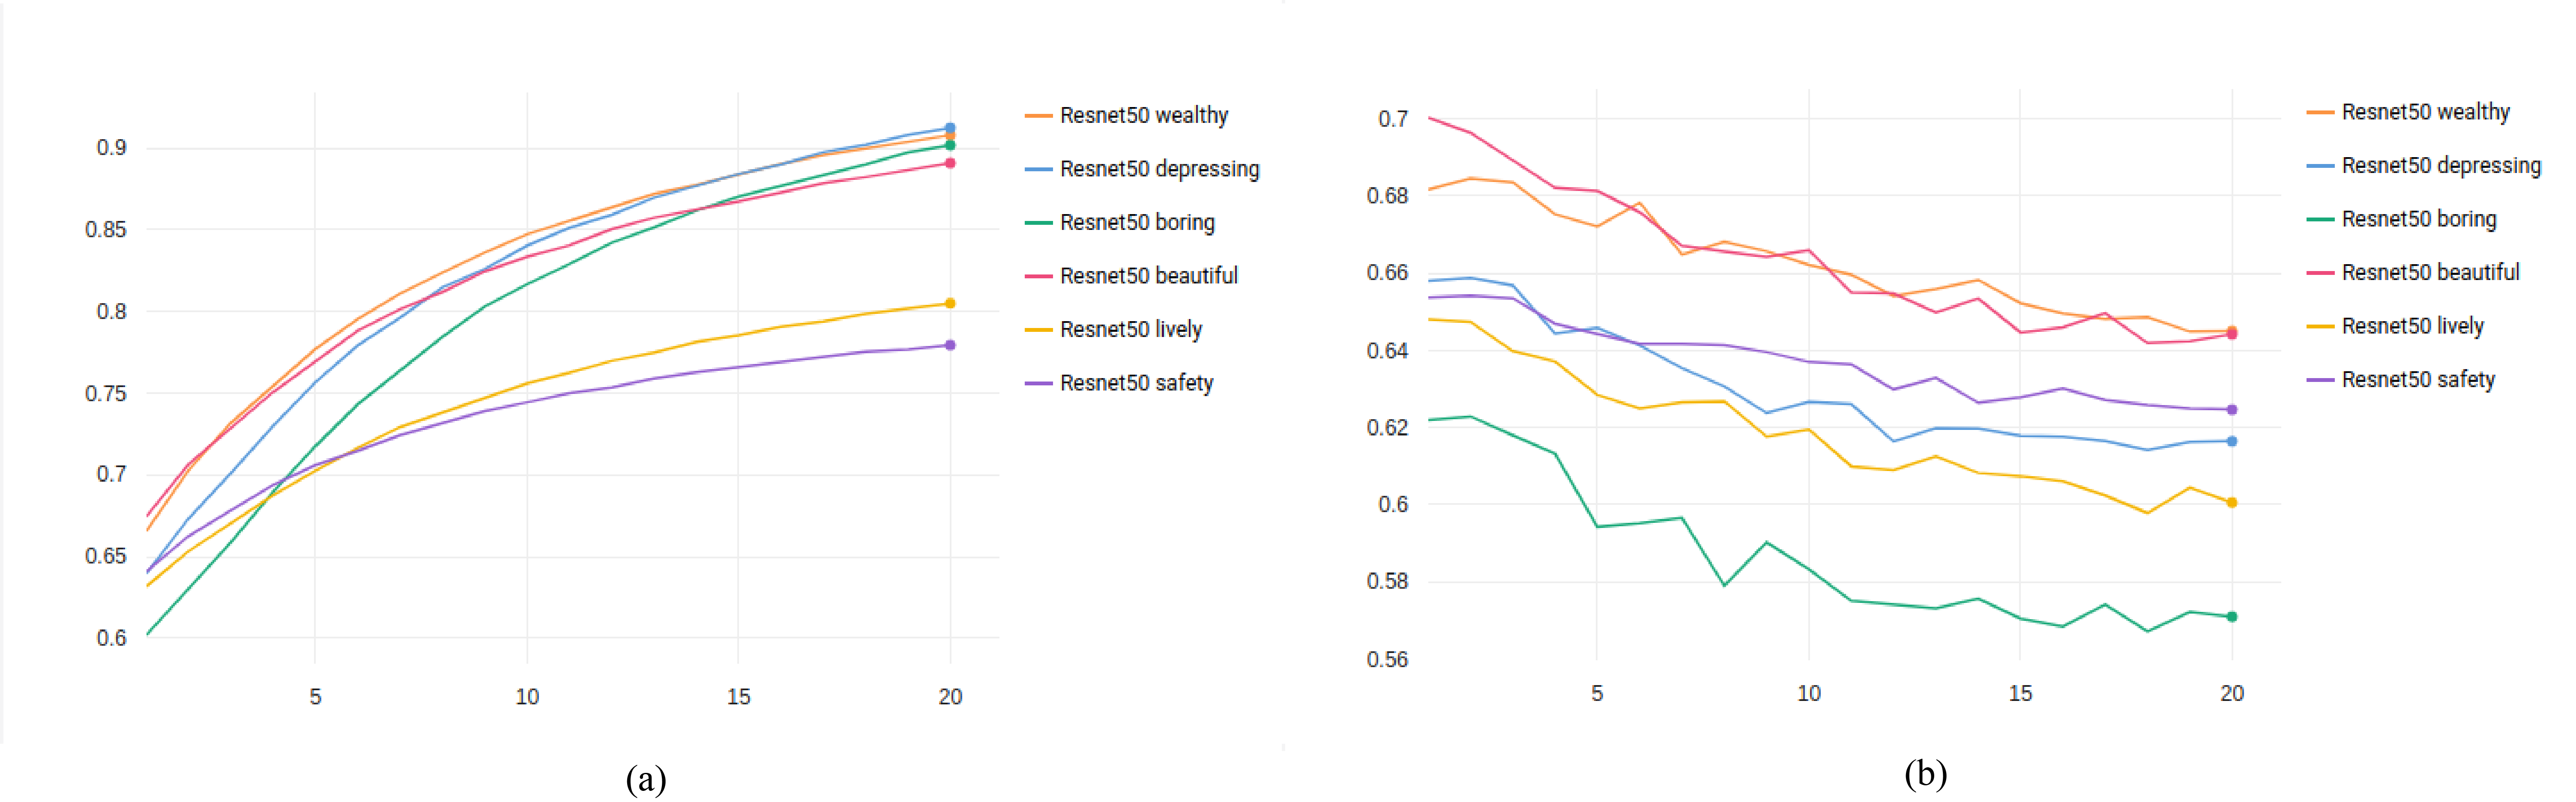
\includegraphics[width=1\textwidth]{./figures/resnet50_graph.png}
	\caption[ResNet Training curves]{
        ResNet50 baseline accuracy vs epoch learning curves on training (a) and validation (b).
        }
	\label{fig:resnet_graph}
	\end{center}
\end{figure}

\begin{figure}[ht]
	\begin{center}
	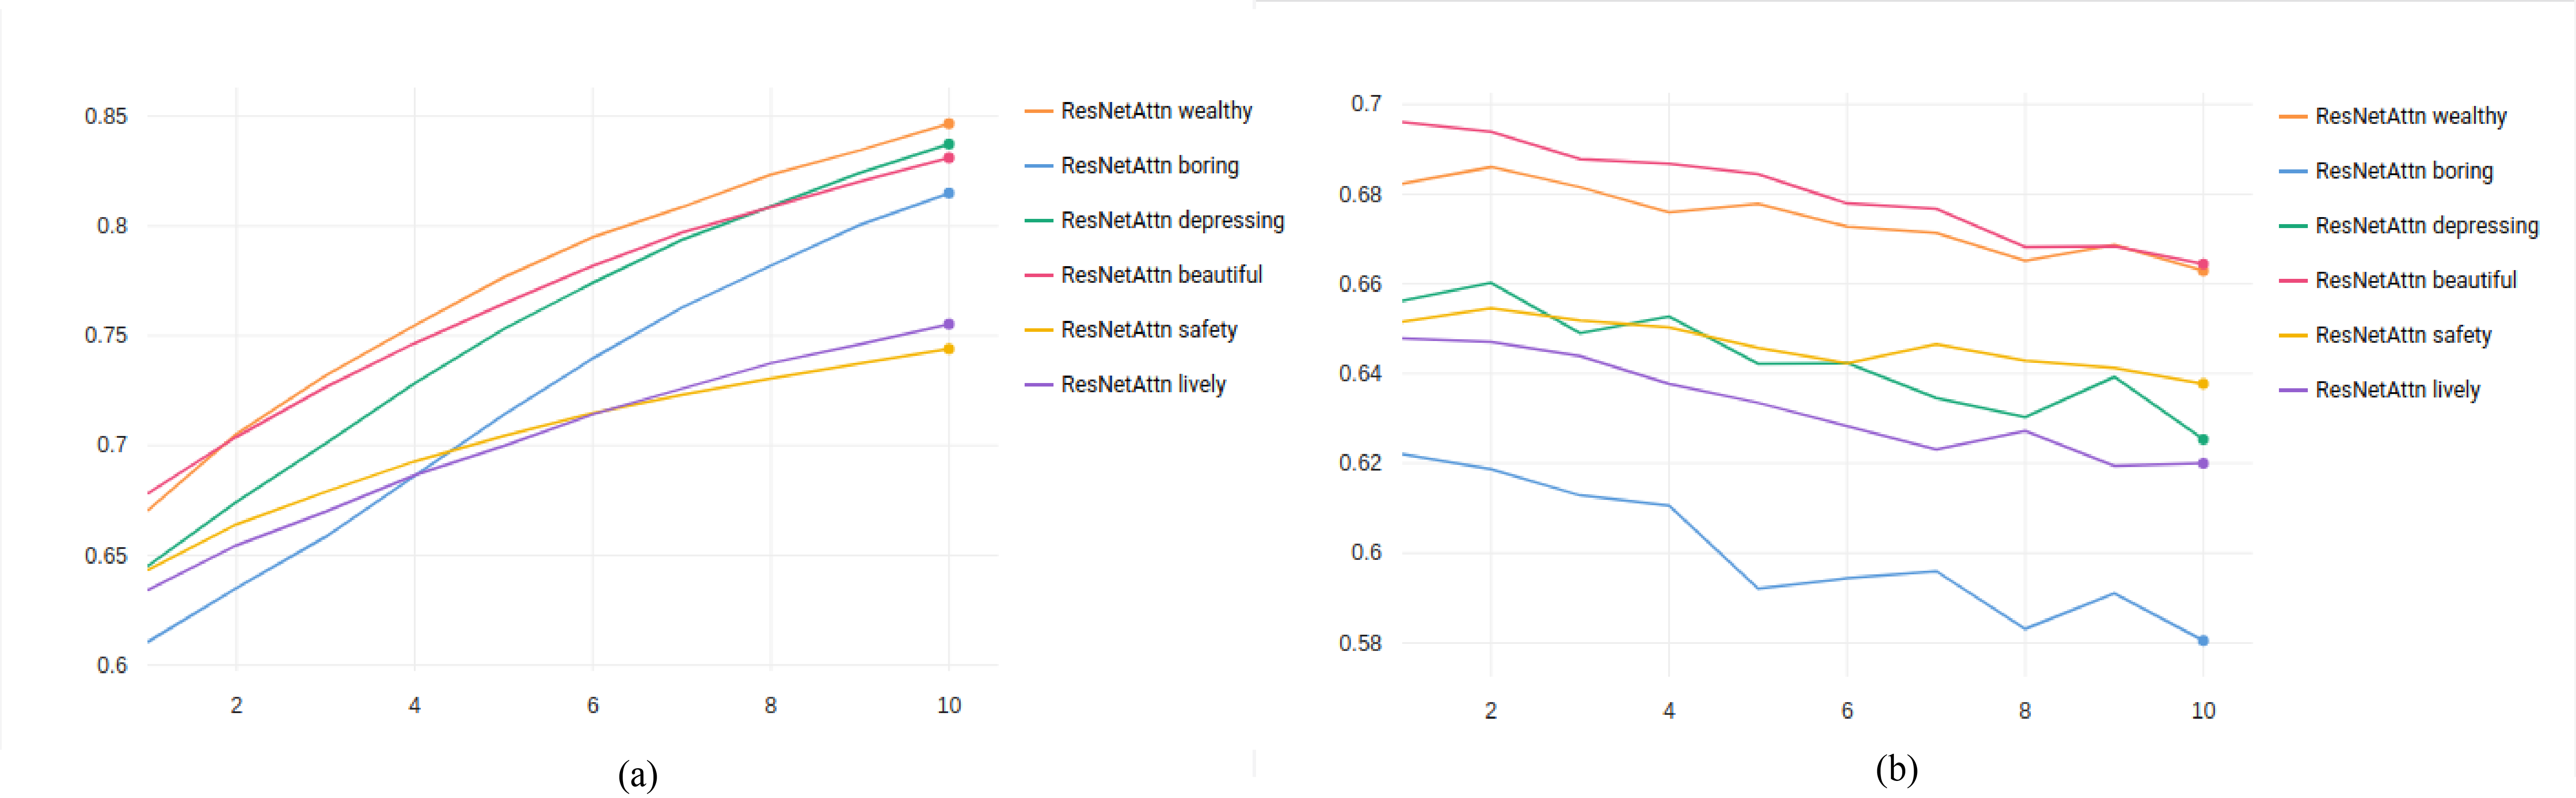
\includegraphics[width=1\textwidth]{./figures/resnet_attn_graph.png}
	\caption[ResNetAttn Training curves]{
        ResNetAttn baseline accuracy vs epoch learning curves on training (a) and validation (b).
        }
	\label{fig:resnet_attn_graph}
	\end{center}
\end{figure}

Replacing the CNN features for semantic segmentation generates a considerable change in training
behavior, with the reduced expressiveness of the segmentation overfitting completely disappears,
which translates to a drop of around 20\% to 30\% accuracy in training, but of only 6\% on validation.

The basic SegRank architecture still reaches convergence after one or two epochs.
Adding the self attention layer makes convergence slightly slower allowing the model reach a higher validation accuracy.


\begin{figure}[ht]
	\begin{center}
	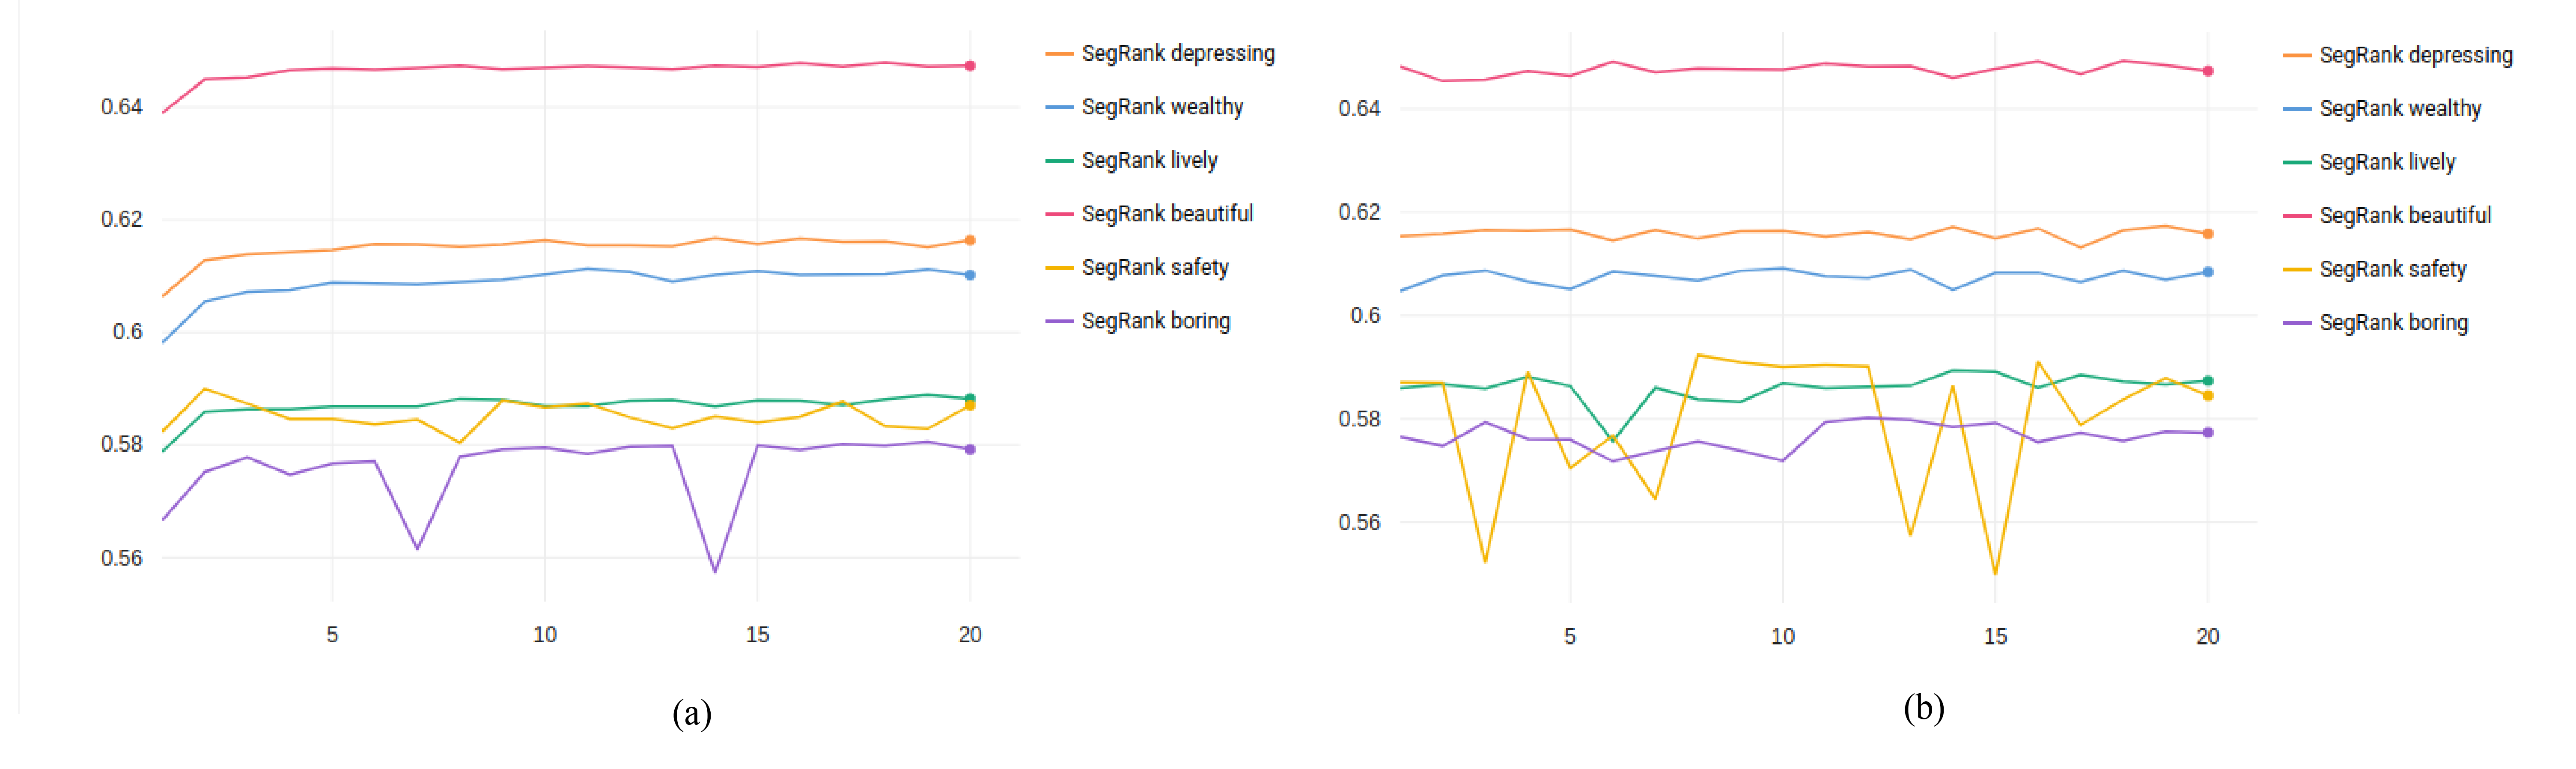
\includegraphics[width=1\textwidth]{./figures/segrank_graph.png}
	\caption[SegRank Training curves]{
        SegRank accuracy vs epoch learning curves on training (a) and validation (b).
        }
	\label{fig:segrank_graph}
	\end{center}
\end{figure}

\begin{figure}[ht]
	\begin{center}
	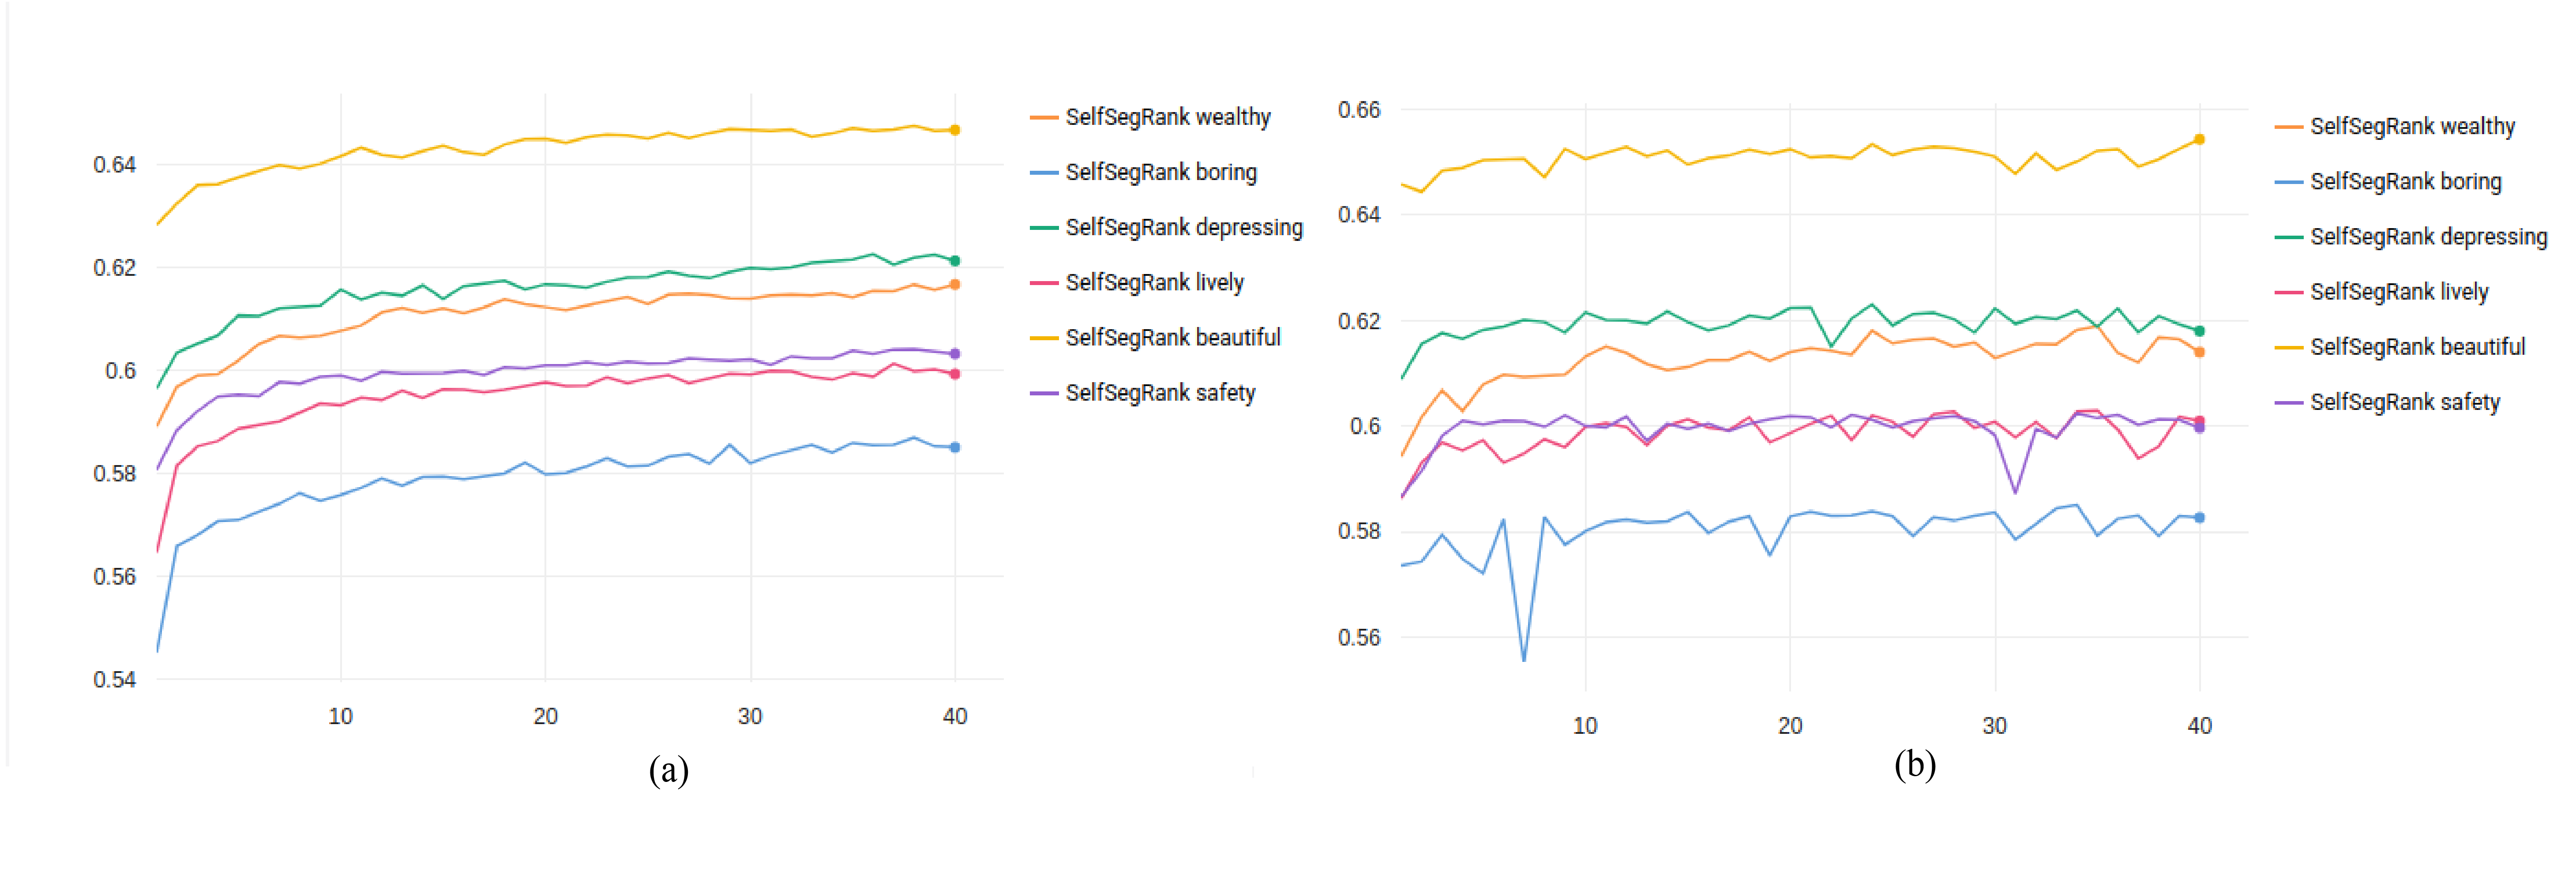
\includegraphics[width=1\textwidth]{./figures/selfsegrank_graph.png}
	\caption[SelfSegRank Training curves]{
        SelfSegRank accuracy vs epoch learning curves on training (a) and validation (b).
        }
	\label{fig:selfsegrank_graph}
	\end{center}
\end{figure}

Interestingly, similar but reduced behavior happens with the AttentionSegRank model,
dropping around 10\% to 20\% accuracy on training and ~2\% on validation.

\begin{figure}[ht]
	\begin{center}
	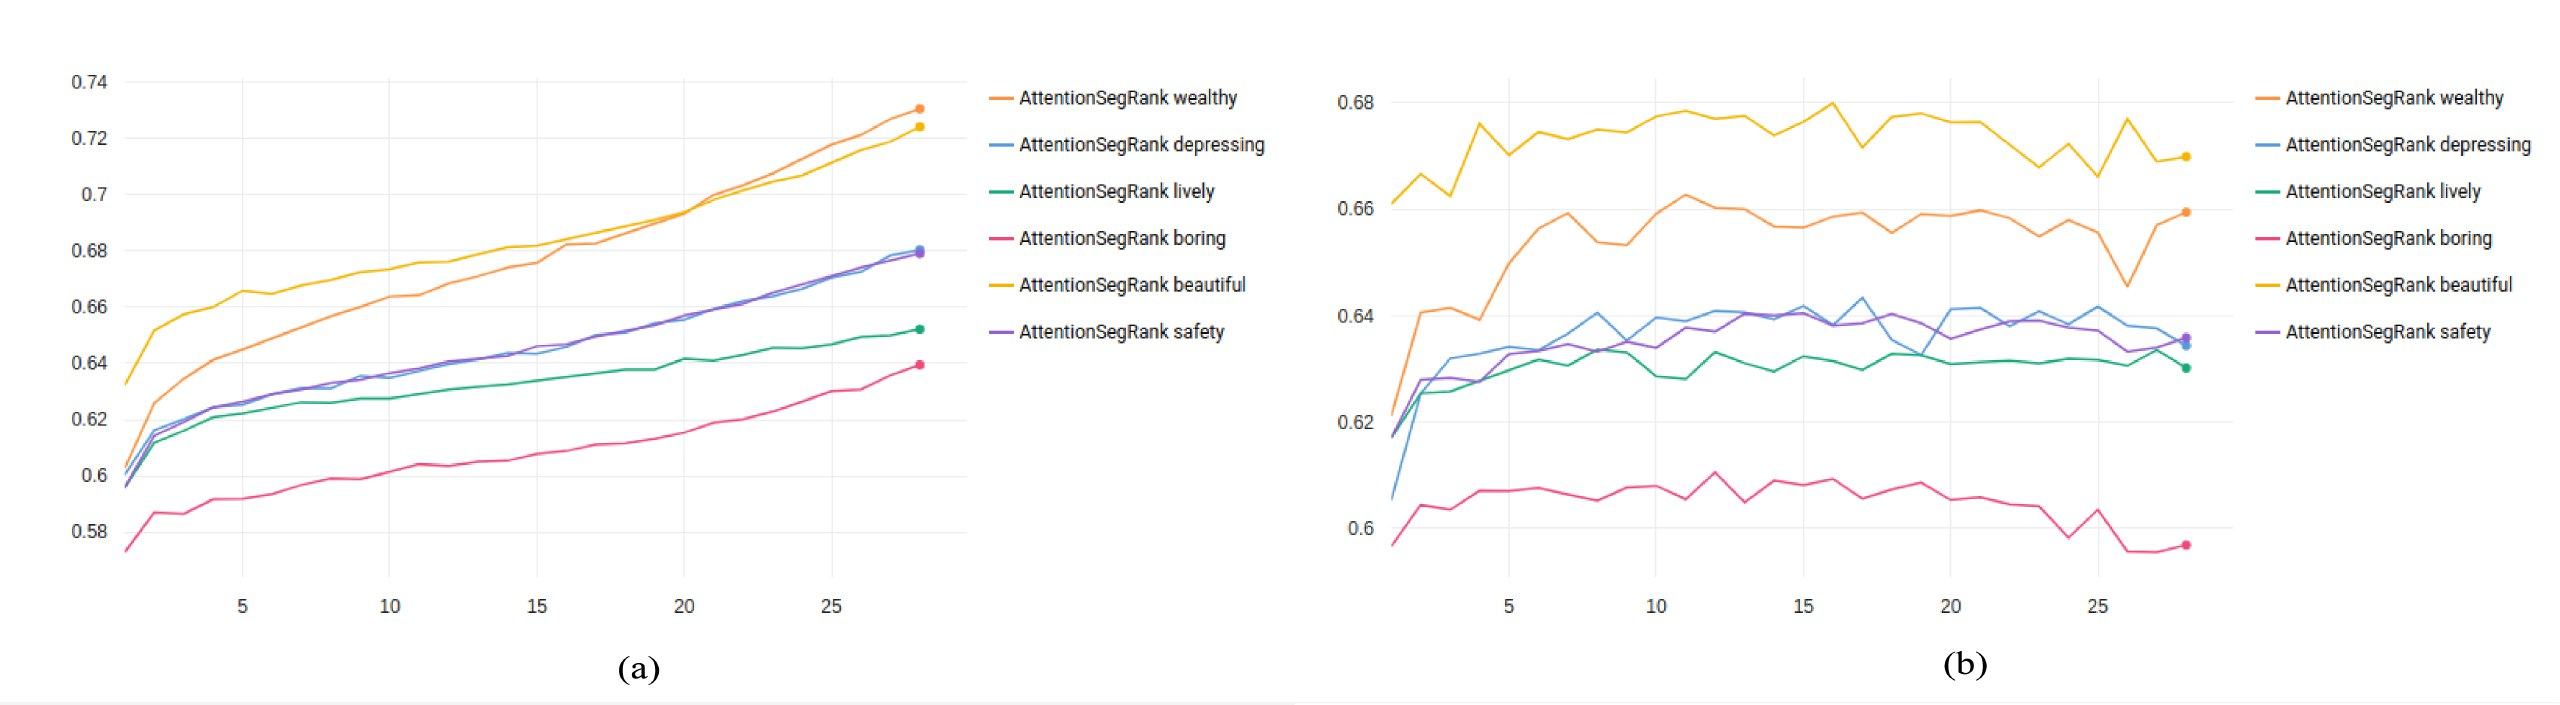
\includegraphics[width=1\textwidth]{./figures/AttentionSegRank_graph.jpg}
	\caption[AttentionSegRank Training curves]{
        AttentionSegRank accuracy vs epoch learning curves on training (a) and validation (b).
        }
	\label{fig:attentionsegrank_graph}
	\end{center}
\end{figure}



As it can be seen on the results of all models, the learning process is consistent through out
the different attributes. The accuracy of the different attributes is also consistent across the
different models, with boring and beautiful being the hardest and easiest tasks to learn respectively
on all models.


\section{Visualization results}
\label{sec:visualization_results}

As was detailed in section \ref{sec:methodology_visualization}, we  derive heatmaps
from the attention weights, which serve as an additional model interpretation
tool on a per instance level. For example, showing the visualization for all attributes on
a single image, shows how the models pay attention to different parts of the image for different
attributes. See figures \ref{fig:segrank_attention}, \ref{fig:vis_sample} for examples.

\begin{figure}[ht]
	\begin{center}
	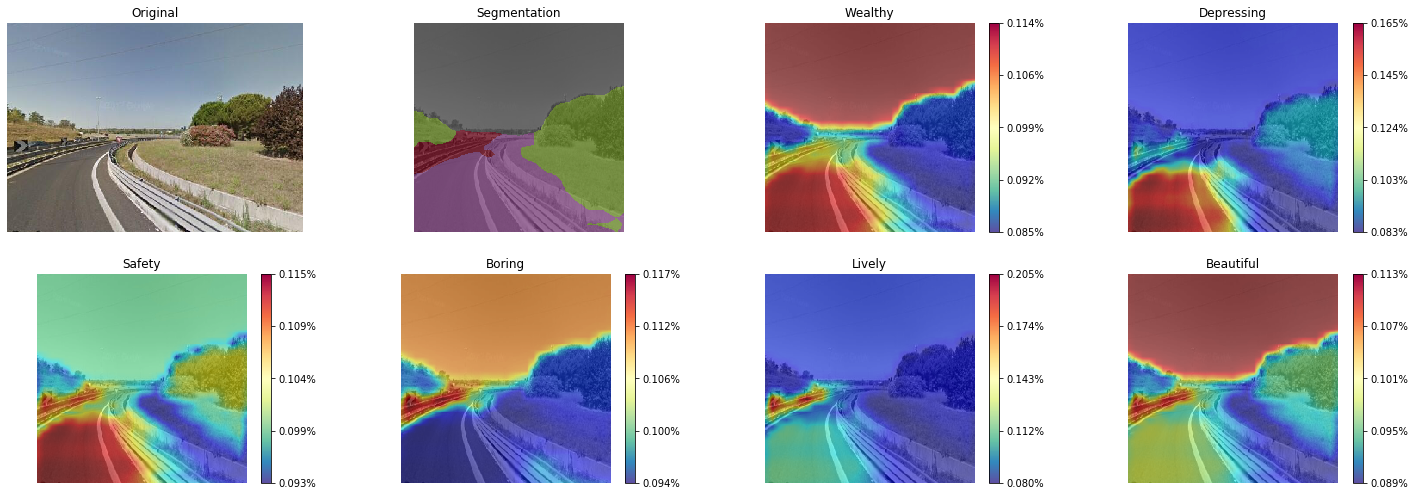
\includegraphics[width=1\textwidth]{./figures/vis_samples(seg_attn).png}
	\caption[Multi attribute Visualization Sample]{
        Attention heatmaps for the AttentionSegRank architecture on all attributes.
        }
	\label{fig:vis_sample}
	\end{center}
\end{figure}

Combining the segmentation with the heatmap allows to see how the attention is distributed
through the different segmentation classes, both qualitatively and quantitatively, as can
be seen in figure \ref{fig:object_attention}.

\begin{figure}[ht]
	\begin{center}
	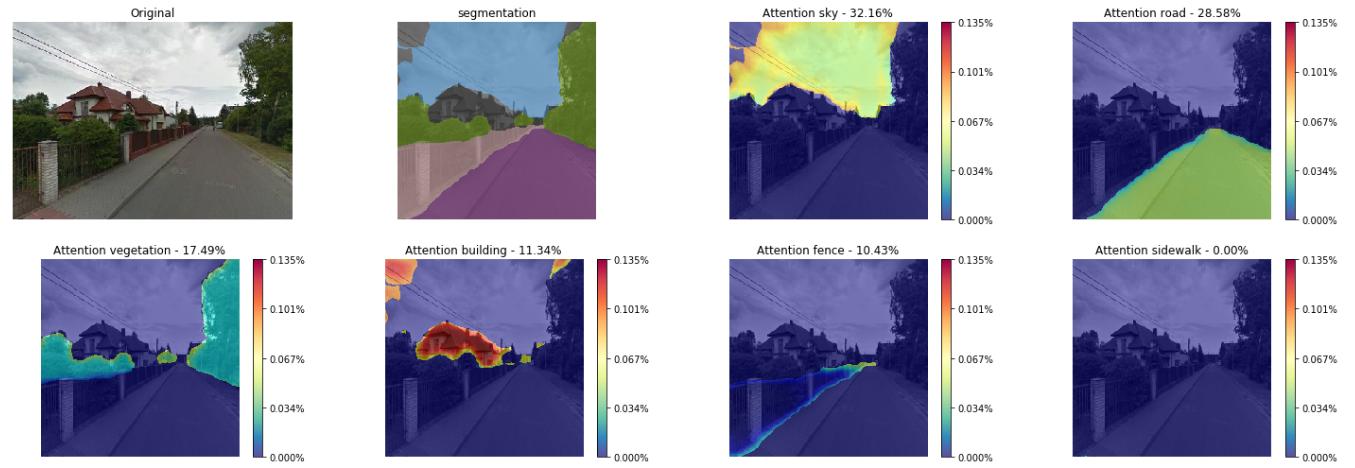
\includegraphics[width=1\textwidth]{./figures/object_attention.png}
	\caption[Attention by segmentation class heatmaps.]{
		Segmentation class separated attention heatmaps for the AttentionSegRank architecture on the boring attribute.
		Only classes present on the segmentation are shown. Percentages indicate the amount of attention given to that
		class.
        }
	\label{fig:object_attention}
	\end{center}
\end{figure}

Is important to note how the three attention models behave differently for the same image, which can be seen by
plotting the heatmaps side by side, as it is shown in figure \ref{fig:model_comparison}

\begin{figure}[ht]
	\begin{center}
	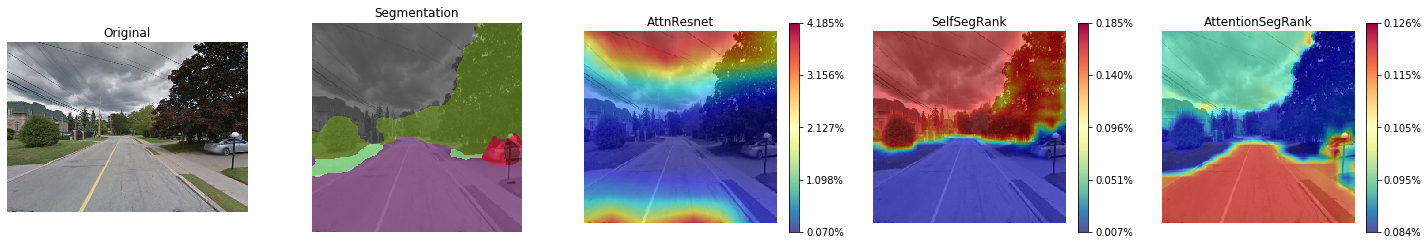
\includegraphics[width=1\textwidth]{./figures/model_comparison.png}
	\caption[Attention by segmentation class heatmaps.]{
		Example of attention heatmaps for the three models on the safety attribute.
		Using segmentation adds significant improvement to the heatmap shapes.
        }
	\label{fig:model_comparison}
	\end{center}
\end{figure}
